% ---------------- RELAZIONE PROGETTO DI PROGRAMMAZIONE AD OGGETTI (OOP) --------
\documentclass[a4paper,12pt]{report}

% ----------------------------- PREAMBLE --------------------------------------- 

\usepackage{lmodern}
\usepackage{alltt, fancyvrb, url}
\usepackage{float}
\usepackage{geometry}
\usepackage{graphicx}
\usepackage[utf8]{inputenc}
\usepackage{hyperref}
\usepackage{amsmath,amssymb,amsthm}
\usepackage{layout}
\usepackage[italian]{babel}
\usepackage[italian]{cleveref}
\usepackage{comment}
\usepackage{microtype}
\usepackage{fancyhdr}
\usepackage[scaled=.92]{helvet}
\usepackage[T1]{fontenc}
\usepackage{lscape}
\usepackage{listings}
\usepackage{color}
\definecolor{dkgreen}{rgb}{0,0.6,0}
\definecolor{gray}{rgb}{0.5,0.5,0.5}
\definecolor{mauve}{rgb}{0.58,0,0.82}

\lstset{frame=tb,
	language=Java,
	aboveskip=3mm,
	belowskip=3mm,
	showstringspaces=false,
	columns=flexible,
	basicstyle={\small\ttfamily},
	numbers=none,
	numberstyle=\tiny\color{gray},
	keywordstyle=\color{blue},
	commentstyle=\color{dkgreen},
	stringstyle=\color{mauve},
	breaklines=true,
	breakatwhitespace=true,
	tabsize=3
}


% hyperref settings
\hypersetup{
	colorlinks=true,
	linkcolor=black, %blue
	filecolor=magenta,      
	urlcolor=cyan,
	pdftitle={Sharelatex Example},
	bookmarks=true,
	pdfpagemode=FullScreen,
}

\geometry{
	a4paper,
	total={170mm,257mm},
	left=20mm,
	top=20mm,
}

% ----------------------------- PREAMBLE END -----------------------------------

\makeindex

\title{\textbf{Visione artificiale}}
\author{Alessandro Pioggia, Luca Rengo, Federico Brunelli, Leon Baiocchi}


\begin{document}
	\makeatletter
	\begin{titlepage}
		\begin{center}
			{\Huge  \@title }\\[3ex] 
			{\large  \@author}\\[3ex] 
			{\large \@date}
		\end{center}
	\end{titlepage}
	\makeatother
	\thispagestyle{empty}
	\newpage
	
	%\maketitle
	
	\tableofcontents
	
	% \input: import the commands from filename.tex to target file.
	
	% \include: does a \clearpage and does an \input.
	
	\newpage
	
	\chapter{Intro}

Idea = cercare di dotare le macchine della vista, si cerca di insegnare ai computer come interpretare le informazioni presenti in immagini e video. 
\section{Che cosa vede un computer?}
Un pc vede una matrice di pixel ed ogni pixel è rappresentato da un numero. Questo è il punto di partenza che ci permetterà di capire che cosa c'è nell'immagine.
\section{Perchè è difficile?}
Punti di vista diversi, occlusione (un oggetto ne copre un altro), distorsione, movimento (a volte può tornare utile), variazioni-intra-classe, sfondo complesso (sfondo non omogeneo, pieno di informazioni che non ci interessano).
\section{Perchè è importante?}
Ha molteplici applicazioni, quali
\begin{itemize}
	\item Sicurezza stradale;
	\item Salute;
	\item Prevenzione del crimine;
	\item Protezione civile;
	\item Divertimento;
	\item Domotica.
\end{itemize}

\newpage

\section{Possibili applicazioni - Panoramica generale}
\begin{itemize}
	\item Misurazione, conteggio, qualità : Hanno in comune il fatto di volere misurare la qualità di un qualche oggetto;
	\begin{itemize}
		\item Misurazione precisa non a contatto : In campo industriale pensiamo ad una catena di montaggio in cui passano prodotti che hanno bisogno di un controllo qualità, che viene svolto da una macchina che sfrutta tecniche di visione artificiale (Controllo delle quantità di liquido in una bottiglietta).
		\item Conteggio di veicoli e persone in una piazza, in generale stime dimensionali;
	\end{itemize}
	\item Elaborazione immagini avanzata
	\begin{itemize}
		\item Miglioramento immagini;
		\item Immagini mediche;
		\item Segmentazione di aree agricoli, utili per individuare le immagini aeree e satellitari.
	\end{itemize}
	\item Riconoscimento
	\begin{itemize}
		\item Classificazione/individuazione di oggetti : Tag inseriti all'interno dell'immagine, Ricerca per somiglianza di immagini, riconoscere segnali stradali;
		\item Riconoscimento persone : punta non solo a classificare, bensì riconoscere univocamente una persona.
	\end{itemize}
	\item Movimento
	\begin{itemize}
		\item Video sorveglianza : individuare un ladro, ritrovare uno zaino perso;
		\item Navigazione e guida autonoma.
	\end{itemize}
\end{itemize}

\section{Strumenti di lavoro}

\subsection{Python}
Standard di fatto per lo sviluppo di software scientifico, tra le altre cose anche di visione artificiale. Linguaggio di alto livello, che ha un certo livello di astrazione, in generale con poche linee, se utilizzate in modo corretto possiamo esprimere concetti piuttosto complessi.

\subsection{OpenCV}
OpenCV è la libreria standard per quanto riguarda la visione artificiale, è sviluppata in C++, però è utilizzata anche da altri linguaggi (quali python).

\subsection{NumPy}
La Lazzaro ce lo ha già spiegato.

\subsection{OpenCV-Python}
Una volta richiamato OpenCV da python, tutte le strutture dati (vettori, punti nelle immagini, ecc.) sono array numPy.

\subsection{Jupyter Notebook}

Ambiente web, in cui vengono scritti piccoli pezzi di codice, immagini e altro al fine di creare dei documenti interattivi.

	
	\chapter{Python}

Python è il Leonardo Di Caprio dei linguaggi di programmazione. Ma perchè?

\section{Descrizione}

\begin{itemize}
	\item Python è un linguaggio ad alto livello, general purpose, può essere utilizzato per qualunque tipo di applicazione;
	\item il codice deve essere facile da leggere, è una prerogativa;
	\item occorrono poche linee di codice per sviluppare anche concetti complessi;
	\item supporta programmazione : oop, imperativa e funzionale;
\end{itemize}

\section{Fun fact}

L'autore, Guido Van Rossum, sceglie il nome python perchè amante del gruppo comico Monty Python, attivo negli anni 70-80. 

\section{Zucchero sintattico}

\subsection{Indentazione}

\begin{lstlisting}
	#Non si puo' cambiare indentazione in un blocco
	print("Salve Cesena")
		print("Salve di nuovo!")
	
	#L'indentazione definisce i blocchi di codice
	if 42 < 0:
		print("ciao")
	print("ciao ma in corsivo")
	
	#andata a capo
	istruzione_molto_lunga = 2 + 5 \
								+ 6 + 7

	#Piu' istruzioni in una singola riga
	print("a"); print("b")
\end{lstlisting}

\subsection{Variabili}

\begin{lstlisting}
	#Le variabili in python non si dichiarano, vengono create automaticamente al momento dell'inizializzazione sono case sensitive, iniziano con una lettera o underscore e i caratteri ammessi sono le Lettere, i numeri e l'underscore (codifica UNICODE)
	
	x = 4
	y = "Visione artificiale"
	print(x, y)
	
	#Assegnamento dello stesso valore a piu' variabili
	
	x = y = z = 90
	
	#Variabili globali e locali
	
	a = "cool" #Variabile globale
	
	def function():
		a = "bad" #Variabile locale alla funzione 
		
	#Se aggiungo global la variabile globale a, definita inizialmente verra' modificata
	def function():
		global a = "bad"
\end{lstlisting}

\subsection{Tipi di dati}

Python è tipizzato, solo che, una volta inizializzata una variabile non abbiamo un modo per specializzare un tipo, una volta assegnato un valore viene definito automaticamente (se scrivo tra "", l'oggetto diventerà una stringa). La variabile non ha tipo, è l'oggetto creato che ha un tipo. Il tipo non è legato alla variabile ma all'oggetto!!! I tipi predefiniti di python sono:
\begin{itemize}
	\item Testo : str
	\item Numeri : int, float, complex
	\item Sequenze : list, tuple, range
	\item Dizionari : dict
	\item Insiemi : set, frozenset
	\item booleani : bool
	\item binari : bytes, bytearray, memoryview
\end{itemize}

\newpage

\begin{lstlisting}
	x = "ciao" #stringa
	x = 20 #int
	x = 20.5 #float
	x = 1j #numero complesso
	x = ["ciao", "come", "stai"] #list
	x = ("ciao", "come", "stai") #tuple
	x = range(5) #range
	x = {"nome" : "Va", "codice" : 17633} #dict
	x = {"ciao", "amico"} #set
	x = frozenset(x) #frozenset, ovvero un set non modificabile
	x = True #bool
	x = b"ABCD" #bytes
	x = bytearray(5) #bytearray
	x = memoryview(bytes(5)) #memoryview
	#con type viene stampato il tipo della variabile
	type(x)
\end{lstlisting}

\subsection{Oggetti, valori, tipi}

Qualunque dato in python è un oggetto, ogni oggetto è caratterizzato da : un tipo, un'identità ed un valore.
Inoltre:
\begin{itemize}
	\item il tipo determina le operazioni che l'oggetto supporta;
	\item l'identità non cambia mai;
	\item Il tipo determina se un oggetto è mutabile o meno;
	\item le variabili sono riferimenti ad oggetti.
\end{itemize}
Python in sè per sè è lento, perchè però ha questo successo? Perchè in un programma sono poche le componenti che devono essere efficienti e sono spesso algoritmi. Gli algoritmi verranno presi da NumPy o altre librerie, che hanno la loro implementazione in C o C++, garantendo massima efficienza.

\begin{lstlisting}
	#L'assegnamento crea un oggetto in memoria di tipo Float, a cui la variabile fa riferimento
	answer = 3.4
	print('Type:', type(answer))
	print('Identity', id(answer))
	print('Value', answer)
	
	#L'assegnamento copia il riferimento dell'oggetto nella nuova variabile
	spam = answer
	print(spam.equals(answer)) #ritornera' True
	 
	 # L'istruzione seguente NON modifica l'oggetto ma crea un nuovo oggetto contenente il risultato e ne assegna il riferimento alla variabile: si puo' osservare infatti che l'identita' dell'oggetto associato a 'answer' e' cambiata, mentre l'identita' di spam e' la stessa
	 answer *= 2
	 print('Identita nuovo oggetto:', id(answer))
	 print('Identita vecchio oggetto :', id(spam))
\end{lstlisting}

\subsection{Alcuni oggetti predefiniti}

Il loro tipo non fa parte dei tipi di base visti prima, hanno un valore particolare.

\begin{itemize}
	\item None : None è l'unico oggetto della classe NoneType, è simile a null ma c'è una differenza sostanziale: quando una variabile è a null significa che non ha un riferimento ad un oggetto mentre il None è un oggetto che esiste in memoria (ne esiste solo uno). Ponendo una variabile = None, la variabile punta a quell'oggetto.
	\item Ellipsis : Sono i puntini di sospensione, è utile in NumPy
	\item NotImplemented : Metodi numerici e di confronto possono restituire questo valore se non implementano l'operazione per determinati operandi.	
\end{itemize}

\begin{lstlisting}
	#Sintassi per oggetto Ellipsis
	x = ...
	y = Ellipsis
	print(x, y)
	#Confronto fra stringa e numero, restituisce notImplemented
	ret = 'testo'._eq_(42)
\end{lstlisting}

\section{Numeri}

I numeri possono essere rappresentati attraverso int, float e Complex, possono essere convertiti utilizzando i relativi costruttori (es: float()).

\section{Stringhe}

Tutti i caratteri messi dentro ad una stringa con triplici apici vengono considerati, non succede la stessa cosa con apici doppi o singoli.
Non esiste il tipo carattere! E' possibile accedere alle stringhe come se fossero array(liste python).

\section{Booleani}
\begin{lstlisting}
	print(10 > 9)
	print(10 == 9)
	print(10 < 9)
	a = 200
	b = 33
	if b > a:
		print("b > a")
	else:
		print("b <= a")
	#Valori convertiti a True
	x = "VA"
	y = 15
	print(bool(x), bool(y), bool("abc"), bool(123))print(bool(["rosse", "verde", "blu"])) #Valori convertiti a False
	print(bool(False), bool(None), bool(0), bool(""))print(bool(()), bool([]), bool({}))
\end{lstlisting}

\section{Operatori aritmetici, di assegnamento, di identità, di appartenenza e bit a bit}

Osservazione sulla divisione : la divisione fra numeri interi avviene attraverso il // (risultato arrotondato all'intero inferiore). Invece usando / ritornerà un float.\\
Per il resto si trova tutto sulle slide del prof oppure sulla documentazione ufficiale di python.

\section{Condizioni if..elif..else}

\begin{lstlisting}
	a = 200
	b = 1
	if b > a:
		print("b>a")
	m = a
		elif b == a:
	print("a=b")
	m = a
		else:
	print("b<a")
	m = b
	print(m)
	# Espressione condizionale
	print("b>a") if b>a else print("b<=a")
	# Due espressioni condizionali a cascata
	print("b>a") if b>a else print("b=a") if b==a else print("b<a")
	# Altro esempio
	print("b>a" if b>a else "b=a" if b==a else "b<a")
\end{lstlisting}

\section{Cicli}


\begin{lstlisting}
	i = 0
	while True:
		i += 1
		if i == 4:
			continue
		print(i)
		if i == 6:
			break
	
	#E' possibile mettere un else fuori da un while, in modo che quando il while diventa falso (solo in questo caso) funziona come una sorta di if
	
	i = 0
	while i < 6:
		print(i)
		i += 1
	else:
		print("Fine del ciclo")
\end{lstlisting}

\begin{lstlisting}
	colori = ["rosso", "verde", "blu"]
	
	for x in colori:
		print(x)
	
	for x in "Visione Artificiale":
		print(x)
	
	for i in range(6):
		print(i)
\end{lstlisting}

\section{Liste}


\begin{lstlisting}
	colori = ['Rosso', 'Verde', 'Blu'] #in alternativa uso il costruttore list()
	print(colori)
	print(type(colori), len(colori))
	print(colori[0]) # Primo elemento
	print(colori[-2]) # Penultimo elemento
	
	for c in colori:
		print(c)
	
	colori[1] = 'Grigio' # Modifica di un elemento
	
	colori.append('Verde')
	colori.remove('Grigio')
	
	 #fa l'append ma con una lista, di solito si utilizza l'operatore +=, che ci da ugualmente la possibilita' di concatenare liste
	
	colori.extend(['Arancione', 'Giallo', 'Viola','Azzurro'])
	print(colori)

	#metodologia con +=
	
	l1 = [1, 2]
	
	#mi permette di creare la lista [1, 2, 3, 4], l'id della lista rimane invariato, perche' la lista e' un oggetto modificabile, quindi non	occorre fare puntare la lista nuova ad un nuovo oggetto
	
	l1 += [3, 4] 
	
	# Esempi di "list comprehension", modo per generare delle liste con la sintassi fra quadre
	
	coloriA = [c for c in colori if c[0]=='A'] #for = tali che
	quadrati = [x*x for x in range(1,10)] #lista di tutti i quadrati degli x che stanno nel range fra 1 e 9
	print(coloriA, quadrati)
\end{lstlisting}

Accesso agli elementi :
\begin{itemize}
	\item indice fra parentesi quadre
	\item Possibile usare indice negativo e intervallo di indici
	\item iterazione con for..in
\end{itemize}
L'operazione * con le liste ripete la stessa lista n volte.

\section{Tuple}

Le tuple non sono modificabili, possono essere create anche attraverso il costruttore tuple().

\begin{lstlisting}
	colori = ('Rosso', 'Verde', 'Blu')
	print(colori)
	print(type(colori), len(colori))
	print(colori[0]) # Primo elemento
	print(colori[-2]) # Penultimo elemento
	
	for c in colori:
		print(c)
	t0 = (3) # N.B. questa non e' una tupla, e' un int
	t0 = () #questa e' invece una tupla
	print(type(t0))
	
	t1 = (3,) # Tupla con un solo elemento
	t2 = (1,2)
	t3 = (4,5,6)
	t = t2 + t1 + t3 # Concatenazione di tuple
	tm = t2 * 3 # Moltiplicazione di una tupla
	print(t, tm)
	
	# Le parentesi si possono omettere
	t1 = 3,
	t2 = 1,2 # Oppure 1,2,
	t3 = 4,5,6 # Oppure 4,5,6,
	print(t1,t2,t3)
\end{lstlisting}

\newpage

\section{Slicing}

Informazioni:
\begin{itemize}
	\item $a[i:j]$ restituisce tutti gli elementi di a con indice k tale che $i \leq k < j$;
	\item $a[:]$ seleziona tutto;
	\item l'espressione estesa : $a[i:j:s]$ comprende lo step, ovvero dice quanti elementi saltare all'interno del range indicato. Posso avere anche uno step negativo, quindi restituisco una stringa ribaltata.
\end{itemize}

\begin{lstlisting}
	a = "Python!"
	print(a[4:6], a[0:2], a[:2]) # on Py Py
	print(a[4:len(a)], a[4:100], a[4:]) # on! on! on!
	print(a[:-3], a[-3:]) # Pyth on!
	print(a[1:-1], a[:]) # ython Python!
	print(a[::2]) # Pto!
	print(a[1::2]) # yhn
	print(a[::-1]) # !nohtyP
	print(a[-3::2]) # o!
	print(a[-1:-4:-2]) # !o
	a = [1, 2, 3, 4, 5, 6, 7, 8, 9]
	print(a[-2::-2]) # [8, 6, 4, 2]
	#Qui notiamo che e' possibile sfruttare anche l'assegnamento, al posto dei primi 3 elementi metto gli altri che ho selezionato
	a[:3] = a[3:]
	print(a) # [4, 5, 6, 7, 8, 9, 4, 5, 6, 7, 8, 9]
	a[::2] = [0]*6 #qui sostituisco tutta la lista, a step 2, con 6 zeri
	print(a) # [0, 5, 0, 7, 0, 9, 0, 5, 0, 7, 0, 9]
	a[3:-3] = []
	print(a) # [0, 5, 0, 7, 0, 9]
	a[:] = a[::-1]
	print(a) # [9, 0, 7, 0, 5, 0]
\end{lstlisting}

\newpage

\section{Insiemi}

Collezione non ordinata e non indicizzata, non può contenere duplicati ma possono essere aggiunti o rimossi elementi (non modificati).

\begin{lstlisting}
	colori = {'Rosso', 'Verde', 'Blu'}
	print(colori)
	print(type(colori), len(colori))
	print('Rosso' in colori)
	
	for c in colori:
		print(c)
		
	#Differenza fra remove e discard : remove da' errore se l'elemento non esiste, discard no, non da' nessun errore
	colori.remove('Verde')
	colori.discard('Giallo') # nessun errore
	colori.add('Azzurro')
	colori.update({'Arancione', 'Viola'})
	print(colori)
	
	# Esempi di "set comprehension", stessa sintassi usata con le liste ma con le graffe
	colori_a = {c for c in colori if c[0]=='A'}
	quadrati = {x**2 for x in range(1,10)}
	print(colori_a, quadrati)
\end{lstlisting}

\section{Dizionari}

Non capita spesso in questo corso.

\begin{lstlisting}
	studenti = {101:"C.Rossi", 103:"M.Bianchi",111:"L.Verdi"}
	print(studenti)
	print(type(studenti), len(studenti))
	if 103 in studenti:
		print(studenti[103])
	studenti[112] = "L.Neri"
	studenti[115] = "A.Rosa"
	for mat in studenti:
		print(mat, studenti[mat])
	for mat, nome in studenti.items(): #items() ritorna chiave-valore
		print(mat, nome)
	for nome in studenti.values(): #values ritorna solo i valori
		print(nome)
	rimosso = studenti.pop(103)
	studenti[103] = rimosso
	# Esempi di "dictionary comprehension"
	studenti_105 = {m: studenti[m] for m in studenti if m<105}
	somme = {(k, v): k+v for k in range(4) for v in range(4)}
	print(studenti_105, somme)
\end{lstlisting}

\section{Funzioni}

I parametri sono riferimenti ad oggetti. Per gli oggetti immutabili, l'effetto è sostanzialmente analogo al passaggio per valore. Per quelli mutabili una funzione può modificare il contenuto di un oggetto.

\begin{lstlisting}
	def stampa_messaggio(): # Definizione funzione
		print("Addio, e grazie per tutto il pesce!")
	stampa_messaggio() # Chiamata della funzione
	
	def calcola(x, y): # Funzione con parametri
		"""Questa e' la docstring di calcola"""
		return x * y
	print(f"Il risultato e' {calcola(6, 7)}.")
	
	# Funzione che sostituisce elementi di una lista, enumerate restituisce un elenco di tuple con indice e valore
	def sostituisci(lista, x, y):
		for (indice, valore) in enumerate(lista):
			if valore == x:
				lista[indice] = y
	
	# Versione piu' "pythonic" della stessa funzione
	def sostituisci2(lista, x, y):
		lista[:] = [y if v==x else v for v in lista]
	
	l = [1, 2, 3, 1, 2, 3]
	sostituisci(l, 2, 0)
	sostituisci2(l, 3, -1)
	print(l)
\end{lstlisting}

\section{Parametri delle funzioni}

\begin{lstlisting}
	def calcola(x, y, z = 1, k = 0):
		return (x * y) / z + k
	print(calcola(2,3), calcola(2,3,3), calcola(2,3,3,-2))
	print(calcola(y=1,x=3), calcola(2,3,k=2),calcola(k=1,x=2,y=3,z=1))
	
	def prodotto(x, *altri_fattori):
		p = x
		for f in altri_fattori:
			p *= f
		return p
	print(prodotto(2), prodotto(6,7), prodotto(2,2,2,2,2))
	
	#* = insieme di parametri senza nome (in questo caso gli argomenti dell'ipotetico corso
	#** = dizionario di parametri con nome
	def Esame(corso, *argomenti, **studenti):
		print("Corso:", corso)
		print("Argomenti:", end=' ')
	for a in argomenti:
		print(a, end=', ')
		print("\nStudenti:")
	for mat in studenti:
		print(mat, studenti[mat])
	Esame("Visione Artificiale", " Python", "NumPy", "OpenCV",M101="C.Rossi", M103="M.Bianchi", M111="L.Verdi")
\end{lstlisting}

\section{Unpacking}

Lo useremo a volte nel passaggio dei parametri.

\begin{lstlisting}
	def calcola(a, b, c):
		return a + b + c
	
	parametri = [4, 18, 20]
	print(calcola(*parametri)) #spacchetta la lista, questo mi permette di passare tre valori separati come argomento della funzione

	a = ["Python", "NumPy", "OpenCV"]
	s = {"M101":"C.Rossi",
		"M103":"M.Bianchi",
		"M111":"L.Verdi"}
	Esame("Visione Artificiale", *a, **s)

	x, y, z = 2, 3, 4 # (x, y, z) = (2, 3, 4)

	a1, a2, a3 = a
	print(a1, a2, a3)
	a1, *r = a #questo serve per spacchettare una lista della quale non ne conosco le dimensioni
	print(a1, r)
	primo, secondo, *altri, ultimo = range(10)
	print(primo, secondo, ultimo, altri)
	
	x, y, _* = a #questo vuol dire che a deve contenere almeno 2 elementi, il primo va in x, il secondo va in y e il resto non mi interessa
\end{lstlisting}

\newpage

\section{Funzioni come oggetti e lambda}


\begin{lstlisting}
	def prodotto(x, y):
		"""Restituisce il prodotto di x e y."""
		return x * y
	
	print(type(prodotto)) # <class 'function'>
	print(prodotto.__name__) # prodottoprint(prodotto.__doc__) # la docstring
	
	def esegui(f, x, y):
		"""Esegue la funzione f su x e y."""
		return f(x, y)
	
	print(esegui(prodotto, 2, 3))
	
	f = lambda x, y: x ** y
	print(type(f)) # <class 'function'>
	print(f.__name__) # <lambda>
	print(f.__doc__) # None
	print(esegui(f, 4, 2))
	print(esegui(lambda x, y: x // y, 9, 2))
\end{lstlisting}

\section{Funzioni predefinite}

\begin{lstlisting}
	s = "Python"
	a = enumerate(s)
	print(list(a))
	# [(0,'P'), (1,'y'), (2,'t'),
	(3,'h'), (4,'o'), (5,'n')]
	
	n = [ord(c) for c in s]
	print(list(n), sum(n), min(n), max(n))# [80, 121, 116, 104, 111, 110] 642 80 121
	
	print(sorted(n))
	# [80, 104, 110, 111, 116, 121]
	
	z = zip(s, n)
	print(list(z))
	# [('P',80), ('y',121), ('t',116),
	('h',104), ('o',111), ('n',110)]
\end{lstlisting}

\newpage

\section{Moduli python}

\begin{lstlisting}
	# Modulo fib.py
	def fibonacci(n): # serie di Fibonacci fino a n
		result = []
		a, b = 0, 1
		while a < n:
			result.append(a)
			a, b = b, a+b
		return result
	
	# Esempi di importazione
	import fib
	print(fib.fibonacci(90))
	
	import fib as f
	print(f.fibonacci(90))
	
	from fib import fibonacci
	print(fibonacci(90))
	
	from fib import fibonacci as f
	print(f(90))
\end{lstlisting}

	
	\chapter{NumPy}

\begin{lstlisting}
	//Hello.java
	import javax.swing.JApplet;
	import java.awt.Graphics;
	
	public class Hello extends JApplet {
		public void paintComponent(Graphics g) {
			g.drawString("Hello, world!", 65, 95);
		}    
	}
\end{lstlisting}
	
	\chapter{Immagini}

\section{Le immagini digitali}

 Una immagine digitale è definita da un insieme di pixel, ogni pixel rappresenta una informazione che viene campionata e quantizzata (ad esempio il colore è quantizzato, in quanto assume un numero finito di valori) misurata da un sensore. Nota : quantizzare significa quantificare. Lavoreremo molto con le immagini grayscale.
 
 \subsection{Caratteristiche di una immagine}
 \begin{itemize}
 	\item Dimensione (numero di pixel in larghezza  = WxH) e risoluzione(DPI);
 	\item formato dei pixel (possono essere o bianchi o neri oppure a colori)
 	\item formati di memorizzazione e compressione;
 	\item occupazione di memoria di una immagine (si misura in funzione dell'ampiezza per altezza per profondità, in sigla si indica come : WxHxDepth)
 \end{itemize}
 
 \subsection{Immagine greyscale con punti di luce}
 
 Vediamo una immagine come una matrice di punti di luce (ogni elemento della matrice rispetta una scala di luminosità).  Ogni pixel della matrice assume un valore, il quale indica la quantità di luce. 
 \begin{itemize}
 	\item valori più alti : maggiore luminosità
 	\item valori più bassi : minore luminosità
 	\item intervalli tipici : Byte[0, 255] e Float[0 = nero, 1 = luce]
 \end{itemize}

 \subsection{Coordinate dei pixel}
 Ci sono due tipi di coordinate:
 \begin{itemize}
 	\item espresse in forma cartesiana (cv.line(img, (4, 0), (3, 6), color));
 	\item espresse in notazione matriciale (img[3, 1] = x).
 \end{itemize}

\subsection{Organizzazione dei pixel in memoria}

I pixel sono quasi sempre organizzati in memoria per righe, ricordando che la memoria dell'elaboratore non è una matrice, bensì un unico vettore unidimensionale di byte.

\section{OpenCV}

Le immagini le definisco come array numpy bidimensionali. Attenzione imread non ritorna un errore o una eccezione nel caso in cui l'immagine non esista, ritorna un None, occorre dunque fare un controllo.

\begin{lstlisting}
	# creazione di un'immagine grayscale 16x15 con un byte per pixel
	
	img1 = np.zeros((15, 16), dtype=np.uint8) # Tutti i pixel a 0
	img2 = np.full((15, 16), 255, dtype=np.uint8) # Tutti i pixel a 255
	img3 = np.random.randint(0, 256, (15, 16), dtype=np.uint8) # Valori dei pixel casuali
	
	# Caricamento di un'immagine grayscale da file (se e' a colori viene convertita)
	# N.B. se il file non esiste non genera un errore ma restituisce None
	
	#il flag indicato ci dice che anche se l'immagine fosse a colori verrebbe convertita in greyscale
	img4 = cv.imread('esempi/mario.png', cv.IMREAD_GRAYSCALE)
\end{lstlisting}

\begin{figure}[htp]
	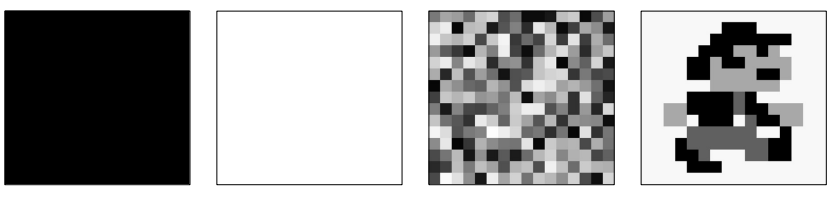
\includegraphics[width=500pt]{./immagini/opencv_images.png}
	\caption{Immagini generate con opencv}
	\label{img:opencv_images}
\end{figure}

\newpage

In seguito viene mostrato come utilizzare slicing e broadcasting per modificare una immagine in python.

\begin{lstlisting}
	a = np.full((15, 16), 255, dtype=np.uint8)	#immagine tutta bianca
	# Slicing e broadcasting
	#partendo dalla terza riga fino alla penultima esclusa, viene fatta la stessa cosa per le colonne
	a[2:-2, 2:-2] = 0		# creo una parte nera, a partire dalla riga di indice 2
	a[4:-4, 4:-4] = 128		# creo una parte grigio chiaro
	a[6:-6, 6:-6] = 64		# grigio con altra tonalita'

	b = a.copy()			
	# Boolean indexing e broadcasting
	mask = b==64 # creo una maschera di bool che conterra' true per tutti i valori di b uguali a 64, dunque sostituisco la parte centrale con il bianco
	b[mask] = 240	#questo array viene esteso attraverso il broadcasting

	c = np.zeros_like(a)	#zeros_like() prende un array e restituisce un array con lo stesso tipo e con le stesse caratteristiche ma tutto a zero
	# Slicing e broadcasting
	c[::2, ::3] = 255

	d = np.zeros((15, 16), dtype=np.uint8)	#immagine nera
	# Integer array indexing e broadcasting
	y = np.array([0, 2, 5, 9, 14])	#array di indici monodimensionale, seleziona le righe sulla quale voglio lavorare
	x = np.arange(0, 16, 2)			#seleziona le colonne che voglio modificare
	#qui sto utilizzando questi array come indici
	d[y[:, np.newaxis], x] = np.arange(50, 255, 50)[:,np.newaxis]
\end{lstlisting}

\begin{figure}[htp]
	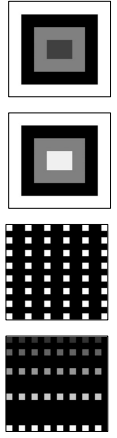
\includegraphics[width=70pt]{./immagini/opencv_images2.png}
	\caption{Immagini generate con opencv}
	\label{img:opencv_images2}
\end{figure}

\section{Immagini a colori: tensori 3D}

Le immagini a colori si modellano mettendo insieme componenti di base (rgb). Una immagine a colori è come se fosse la sovrapposizione di 3 immagini con una determinata scala di valori. Quindi abbiamo che le immagini a colori sono definite da array tridimensionali, la profondità è data dai canali. Sovrapponendosi fra loro dunque, i canali conferiscono il colore all'immagine.

\subsection{Modello RGB}

Ci sono tanti modelli, in questo corso vediamo il minimo indispensabile per capire di cosa si tratti. Il modello di base è l'RGB, è utilizzato ad esempio per generare colore nei monitor, è un modello additivo dal momento che combinando il verde il blu e il rosso si ottiene tutta la varietà di colori. Alla fine abbiamo questi 3 colori ed ogni colore lo possiamo immaginare come un punto in uno spazio tridimensionale (asse del rosso, asse del verde e asse del blu). Per effettuare operazioni di riconoscimento degli oggetti (somiglianza fra colori), lo spazio euclideo del cubo RGB non va bene, perchè i colori che sono simili non sempre sono vicini.

\subsection{Coordinate dei pixel}
Notazione:
\begin{itemize}
	\item cartesiane : pixelpos = (14, 3, 1), sto indicando x, y e canale;
	\item matriciale : img[14, 4, 0], sto indicando r, c, canale.
\end{itemize}

\subsection{Ordine dei canali}

L'ordine dei canali sfruttato normalmente è RGB ma attenzione! Open CV utilizza il modello BGR (B = 0, G = 1, R = 2). In caso di cambio ordine occorre effettuare delle modifiche.

\subsection{Quale è l'ordine dei pixel in memoria?}

Quasi sempre viene utilizzato un canale in modo contiguo. 

\newpage

\section{Caricamento di immagini a colori}

\begin{lstlisting}
	# Creazione di un'immagine 16x20 a 3 canali con valori di tipo byte (3 byte per pixel)

	img1 = np.zeros((20, 16, 3), dtype=np.uint8) # Pixel a 0
	img2 = np.full((20, 16, 3), 255, dtype=np.uint8) # Pixel a 255
	img3 = np.random.randint(0, 256, (20, 16, 3), dtype=np.uint8) # Pixel casuali

	# Caricamento di un'immagine da file (formato BGR)
	# N.B.: se il file non esiste non genera un errore ma restituisce None
	img4 = cv.imread('esempi/mario-c.png')
\end{lstlisting}


\begin{lstlisting}
	# Caricamento di un'immagine da file (formato BGR)
	m = cv.imread('esempi/mario-c.png')
	
	# Crea tre immagini BGR ciascuna con valori solo in un canale e gli altri due a zero
	b, g, r = m.copy(), m.copy(), m.copy()
	#Qui voglio azzerare tutti i canali tranne 1, in modo da ottenere delle immagini monocolore. Lo faccio sfruttando l'ellipsis notation e lo slicing.
	b[...,1:3], g[...,0:3:2], r[...,0:2] = 0, 0, 0
	
	# Crea tre immagini BGR ciascuna corrispondente alla somma di due canali
	c, m, y = b+g, b+r, g+r
\end{lstlisting}

\begin{figure}[htp]
	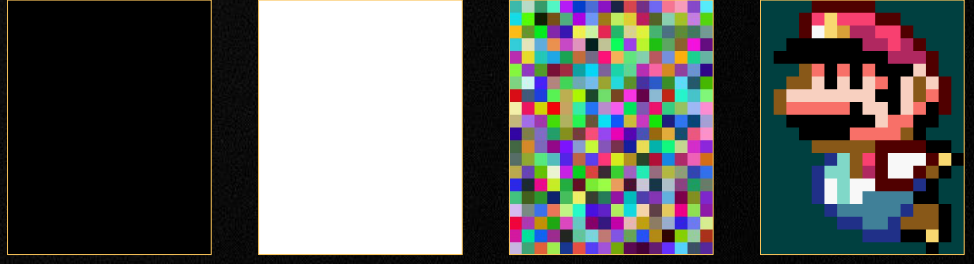
\includegraphics[width=200pt]{./immagini/opencv_images_c1.png}
	\caption{Prime immagini a colori}
	\label{img:opencv_images_c1}
\end{figure}

\begin{figure}[htp]
	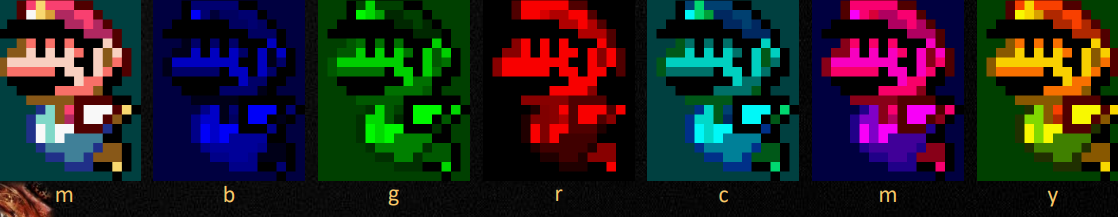
\includegraphics[width=200pt]{./immagini/opencv_images_c2.png}
	\caption{Altre immagini a colori}
	\label{img:opencv_images_c2}
\end{figure}

\newpage

\section{Array numpy tridimensionali}

\begin{figure}[htp]
	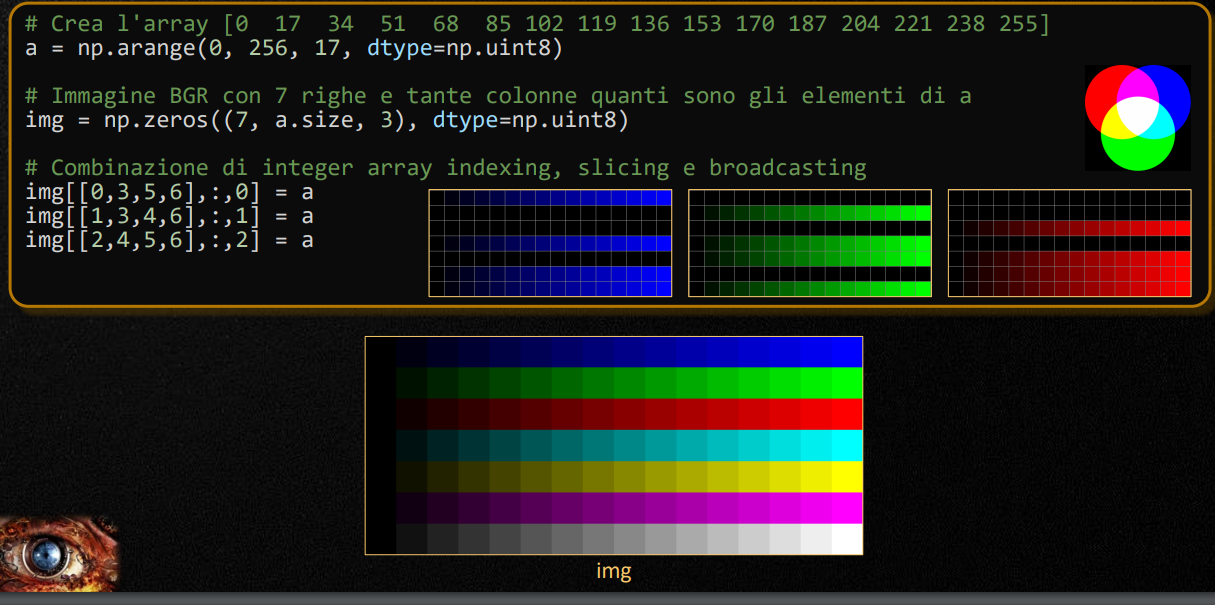
\includegraphics[width=\linewidth]{./immagini/opencv_images_c3.png}
	\label{img:opencv_images_c3}
	\caption{Indicizzazione di array di interi, nell'ultima parte sto dicendo : nel canale 0, su tutte le colonne e su una serie di righe, copio la configurazione definita nel canale a. Faccio la stessa cosa sul canale 1 e 2.}
\end{figure}

\begin{figure}[htp]
	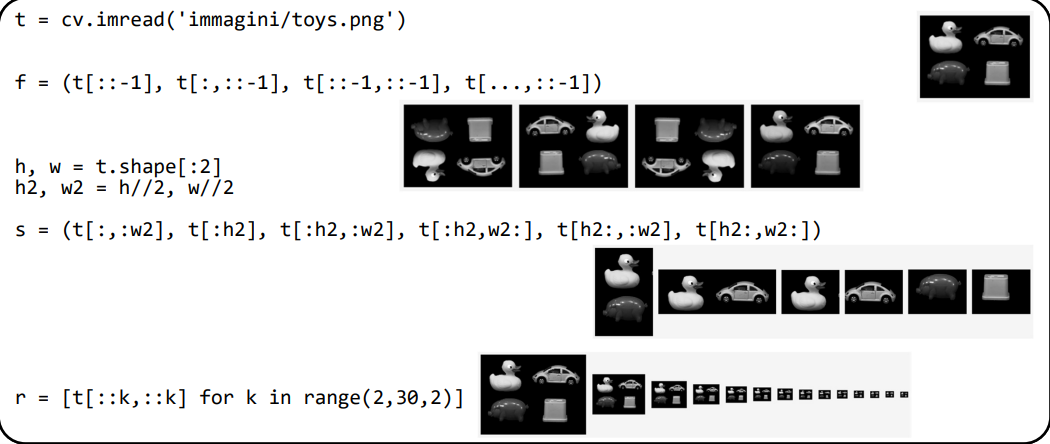
\includegraphics[width=\linewidth]{./immagini/opencv_images_c4.png}
	\caption{Qui utilizziamo lo slicing per fare a fette le immagini. Nel primo caso sto generando una tupla di array numpy}
	\label{img:opencv_images_c4}
\end{figure}

\newpage

\section{Istruzione shape}

\begin{lstlisting}
	t = cv.imread('path')
	
	t.shape #mi mostra la shape dell'immagine : (righe, colonne, canali)
	
	#un amateur fa cosi'...
	
	w = t.shape[1] #numero delle righe
	h = t.shape[0] #numero di colonne
	
	print("Dimensione immagine", w, x, h)
	
	#un super python expert giga chad fa invece cosi'!
	
	h, w, c = t.shape #questo perche' conosco lo scompattamento delle tuple
	
	h, w = t.shape #faccio cosi' se il valore del canale non mi interessa
	
\end{lstlisting}

\section{Rappresentazioni HSV HSL}

Introduciamo due modelli di colori più comodi per noi esseri umani. Sono basate su:
\begin{itemize}
	\item Hue(tinta) : è un angolo;
	\item Saturation(saturazione) :  quanto il colore è bello vivo, va dai colori spenti ai più accesi;
	\item Value o lightness: dice quanta luce c'è nel colore, va dal nero al bianco.
\end{itemize}

\subsection{Differenze HSV e HSL}

In HSV i colori più saturi hanno luminosità 1, mentre nell'HSL 0.5. Ci sono altre caratteristiche che non verranno affrontate nello specifico in questo corso.

\subsection{Modifica ai canali HSL}

Creo un mapping, sfruttando la scala greyscale, fra tutti i possibili angoli (che corrispondono ai colori), consideriamo i valori fra 0 a 255. Per quanto riguarda la saturazione, nel mapping greyscale, si vede in base all'oggetto più luminoso (colore più spento = colore poco saturo, colore più accesi = colore molto saturo). Alla fine della fiera, in questa immagine viene mostrato come determinare i valori H, S ed L attraverso un intelligente mapping  della scala greyscale. Ad esempio, se eseguo una somma sullo HUE sto in realtà ruotando la ruota dei colori, per quello utilizziamo le notazioni in radianti.

\begin{figure}[htp]
	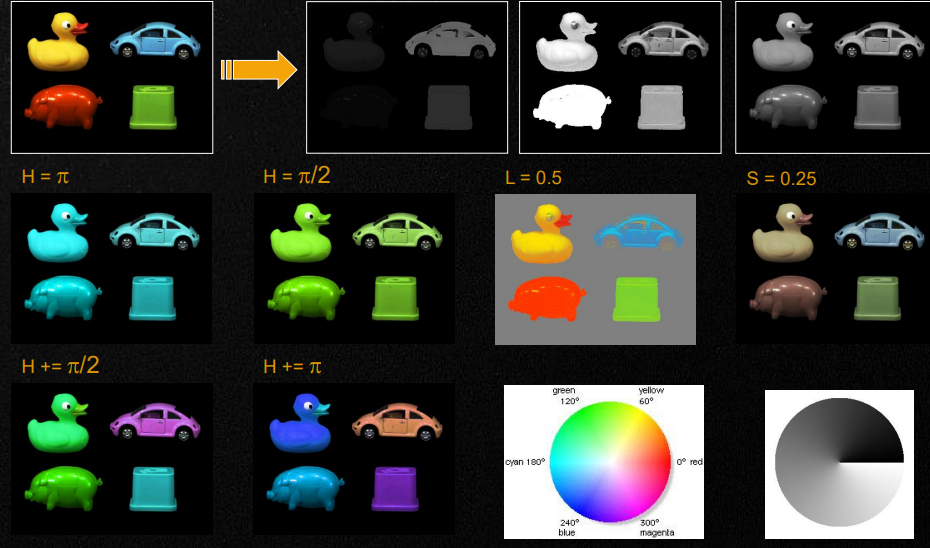
\includegraphics[width=\linewidth]{./immagini/opencv_images_c5.png}
	\caption{Qui utilizziamo lo slicing per fare a fette le immagini. Nel primo caso sto generando una tupla di array numpy}
	\label{img:opencv_images_c5}
\end{figure}

\subsection{HSV e HSL in python/openCV}

La funzione cv.cvtColor(originale, CONV) effettua la conversione del formato del colore, lo si fa specificando una costante come secondo argomento. Attenzione! In python invece di HLS viene considerato HSL.

\begin{lstlisting}
	originale = cv.imread('immagini/toys.png')
	# Converte in HLS
	hls = cv.cvtColor(originale, cv.COLOR_BGR2HLS)
	# Separa i tre canali in 3 immagini grayscale
	h, l, s = cv.split(hls)
	
	# Modifica alcuni dei valori HLS
	# Dimezza la luminosita' di tutti i pixel
	
	l1 = l//2
	
	# Valore di saturazione 64 per tutti i pixel
	
	s1 = np.full_like(s, 64)
	
	# Riunisce i canali e converte in BGR
	#merge e' il corrispettivo di merge, vuole un solo parametro e deve essere una tupla
	
	risultato = cv.cvtColor(cv.merge((h, l1, s1) 
\end{lstlisting}

\begin{figure}[htp]
	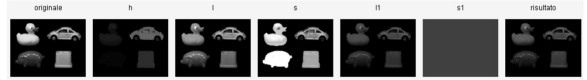
\includegraphics[width=300pt]{./immagini/opencv_images_c6.png}
	\label{img:opencv_images_c6}
\end{figure}

\begin{lstlisting}
	s = [0, 64, 128, 192, 255] # 5 livelli di saturazione
	
	# 18 valori di luminosita' in ogni colonna, np.tile permette di replicare tutte le volte che voglio un array, creando un array piu' grande
	v = np.tile(np.arange(255, -1, -15, np.uint8)[:,np.newaxis], (1, 18))
	
	# 18 valori di hue in ogni riga
	h = np.tile(np.arange(0, 180, 10, np.uint8), (18, 1))
	
	# Combina i 3 canali (si poteva usare anche cv.merge)
	hsv = [np.dstack((h, np.full_like(h, x), v)) for x in s]
	hls = [i[...,[0,2,1]] for i in hsv] # Scambia gli ultimi due canali
\end{lstlisting}


\begin{figure}[htp]
	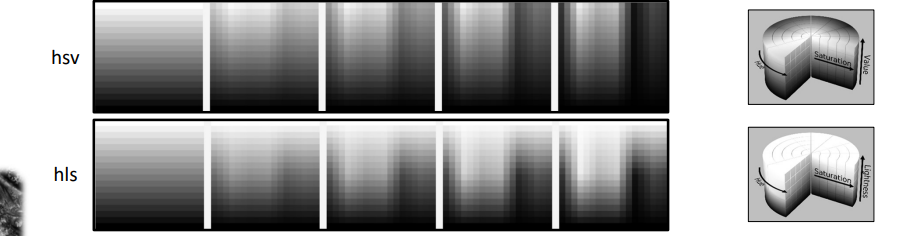
\includegraphics[width=\linewidth]{./immagini/opencv_images_c7.png}
	\label{img:opencv_images_c7}
\end{figure}

\newpage

\section{Istogramma di una immagine grayscale}

Un istogramma è un grafico che ci dice quanti pixel dentro all'immagine ci sono per ciascuno dei possibili livelli di grigio. Nell'esempio abbiamo a sinistra una immagine con 1 byte per ogni pixel, quindi ogni immagine può avere valori da 0 a 255. Il nostro istogramma avrà 255 possibili colonne, da 0 a 255 e l'altezza di ogni colonna di questo istogramma sarà uguale a quanti pixel di quel livello di grigio ci sono in tutto nell'immagine. L'istogramma nelle immagini è importante, perchè permette di estrarre informazioni interessanti, quali:
\begin{itemize}
	\item se la maggior parte dei valori sono solo condensati in una zona, l'immagine ha uno scarso contrasto;
	\item se nell'istogramma sono predominanti le basse intensità, l'immagine è molto scura.
\end{itemize}



\begin{figure}[htp]
	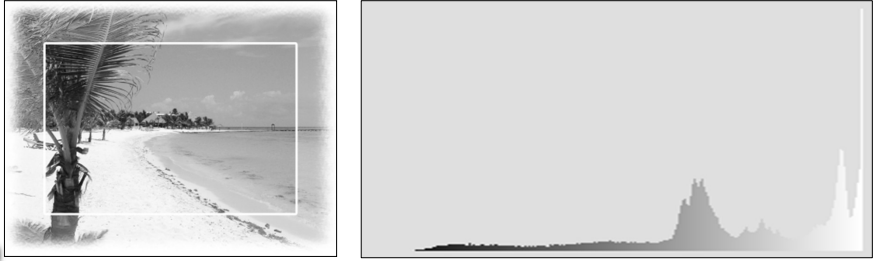
\includegraphics[width=\linewidth]{./immagini/istogramma_spiaggia.png}
	\label{img:istogramma_spiaggia}
\end{figure}


\section{Calcolo istogramma}

\begin{lstlisting}
	
	#da non fare in un progetto reale, perche' e' lentissimo, il python non e' adatto ad eseguire dei cicli
	def calc_hist_py(img):
		h = np.zeros(256, dtype=int)
		#np.nditer e' un iteratore
		for p in np.nditer(img):
			h[p] += 1	#questo mi alza la colonnina dell'indice p
		return h
	
	#np.histogram(immagine, numero di elementi dell'istogramma, range dei valori) e' generale, non specifico per le immagini. Questo metodo restituisce una tupla con 2 valori, il primo valore e' l'array dell'istogramma, il secondo valore della tupla e' l'elenco dei range. Per questo e' stato considerato solo l'elemento di indice 0.
	def calc_hist_np(img):
		return np.histogram(img,256,[0,256])[0]
	
	#cv.calcHist() e' specifico per le immagini, calcola tanti istogrammi in un colpo solo. Noi gli passiamo (lista python, canale(lista), ).  Restituisce un array bidimensionale, il prof usa squeeze() che elimina le dimensioni ad 1 (dal momento che sto passando una singola immagine).
	def calc_hist_cv(img):
		return cv.calcHist([img], [0], None, [256], [0, 256]).squeeze()
\end{lstlisting}

\begin{figure}[htp]
	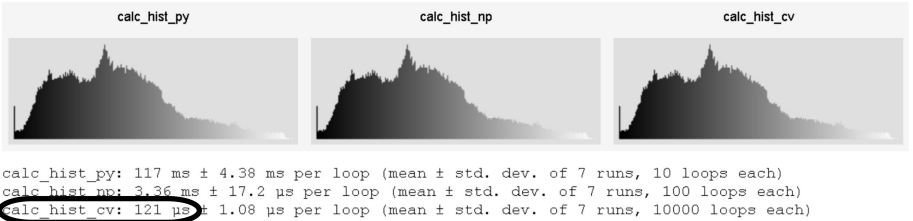
\includegraphics[width=\linewidth]{./immagini/istogrammi.png}
	\label{img:istogrammi}
\end{figure}

\newpage

\section{Analisi dell'istogramma}

A livello di contenuto dell'immagine, quando non è troppo complessa, è possibile ricavare anche legate agli oggetti. Ad esempio si può notare la separazione fra una torre ed il cielo, questo tipo di istogramma è di tipo bimodale. 

\section{Operazioni sui pixel}

\subsubsection{Su una singola immagine}
\paragraph{Formula} $I'[y, x] = f(I[y, x])$\\
Consistono nell'applicazione di una funzione al valore di ciascun pixel. Ciò mi produrrà una immagine delle stesse dimensioni e il valore di ciascun pixel della nuova immagine dipenderà \textbf{unicamente} dal valore del corrispondente pixel nell'immagine di partenza. Esempi:
\begin{itemize}
	\item Variazione della luminosità; 
	\item variazione del contrasto;
	\item conversione da livelli di grigio a (pseudo) colori;
	\item binarizzazione con soglia globale.
\end{itemize}


\subsubsection{Su più immagini}
\paragraph{Formula} $I'[y, x] = f(I_1[y, x], I_2[y, x], ...)$ \\
In questa applicazione vengono prese più immagini (tutte con le stesse identiche dimensioni), la nostra funzione prende il valore di un pixel e lo distribuisce fra più immagini, ritornando poi una singola immagine.


\section{Variazione luminosità e contrasto}

\subsubsection{Formula classica}

$f(v) = \alpha \cdot v + \beta$ \\\\
$v$ è un valore di luminosità per un'immagine, per capirci è quello che nella sezione precedente abbiamo chiamato $I[y, x]$. $\alpha$ controlla il contrasto, $\beta$ controlla la luminosità e vogliamo che il valore di output sia un byte (per garantirlo si va a tagliare, andandolo a forzare nell'intervallo [0, 255]). Ponendo $\alpha = 1$ e $\beta = 0$ viene la funzione identità.

\newpage

\section{Gamma correction - funzione non lineare}

Modo non lineare per aumentare la luminosità dei toni scuri o la luminosità dei toni chiari.
\subsection{Formula}

$f(v) = (\tfrac{v}{255})^{\gamma} \cdot 255$ \\\\
\begin{itemize}
	\item se $\gamma < 1$ aumenta la luminosità dei toni scuri;
	\item se $\gamma > 1$ diminuisce la luminosità dei toni chiari; 
	\item se $\gamma = 1$ otteniamo la funzione identità.
\end{itemize}
In prima istanza normalizziamo il numero di pixel fra 0 ed 1 (attraverso la frazione, 0 corrisponde al nero, 1 corrisponde al bianco). Anche elevando alla $\gamma$ il valore resterà comunque compreso fra 0 e 1, moltiplicando per 255 infine otterrò un valore compreso nell'intervallo [0, 255].

\section{Lookup table (LUT)}

Concetto molto importante quando si lavora con funzioni che si applicano sul singolo pixel. In generale la lookup table rappresenta un concetto molto utilizzato in informatica, è una tabella in cui vado a cercare qualcosa che mi interessa. Idea di base: faccio il calcolo una volta e lo salvo nella table, in modo da evitare inutili sprechi computazionali. In questo caso ho in memoria un array di 256 byte, determinando applicando la funzione $f(v)$ su 256 valori distinti.

\begin{figure}[htp]
	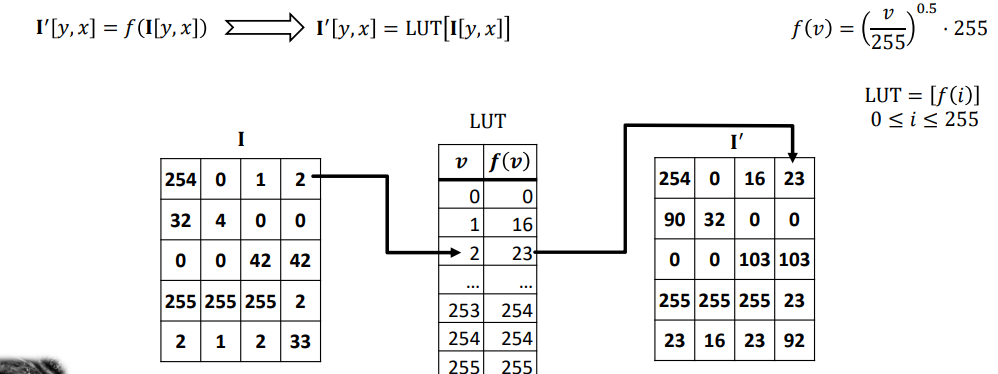
\includegraphics[width=\linewidth]{./immagini/LUT.png}
	\label{img:LUT}
\end{figure}

\newpage

\section{LUT in python/numpy/OpenCV}

\begin{lstlisting}
	# Un esempio di funzione f (Gamma correction per un certo valore di )
	y = 0.5	
	# Calcolo di un singolo valore di f
	f = lambda p: 255 * (p/255.0)**y
	# Calcolo di f su tutti i valori di un array NumPy, impongo .astype(np.uint8) perche' altrimenti numpy restituisce un risultato in virgola
	f_np = lambda a: f(a).astype(np.uint8)
	# Calcolo dell'array LUT
	lut = f_np(np.arange(256))
	# Una semplice implementazione Python senza lookup table
	def applica_py_f(img):
		res = np.empty_like(img)	#creo una immagine vuota
		h, w = res.shape			
		#applico la funzione f al singolo valore del pixel, ripetuto per tutti i pixel
		for y in range(h):			#vado da 0 fino ad h - 1 
			for x in range(w):		#vado da 0 fino a w - 1
				res[y,x] = f(img[y,x])
		return res
\end{lstlisting}

\begin{lstlisting}
	# Semplice implementazione Python con LUT
	def applica_py_lut(img):
		res = np.empty_like(img)
		h, w = res.shape
		for y in range(h):
			for x in range(w):
				res[y,x] = lut[img[y,x]]
		return res
	# Implementazione NumPy senza LUT, applica la funzione f su tutto l'array, prima l'ho usato per calcolare la LUT ma nulla mi vieta di applicare questa funzione su un array bidimensionale (in questo caso la mia immagine).
	def applica_np_f(img):
		return f_np(img)
	# Implementazione NumPy con LUT, sto sfruttando l'indicizzazione con img, un array bidimensionale di interi
	def applica_np_lut(img):
		return lut[img]
	# Funzione LUT di OpenCV
	def applica_cv_lut(img):
		return cv.LUT(img, lut)
\end{lstlisting}

\begin{figure}[htp]
	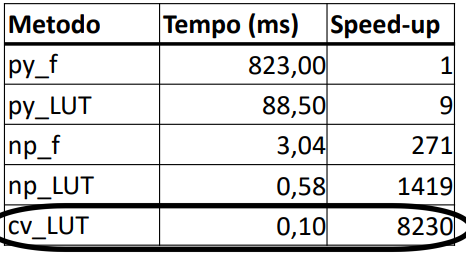
\includegraphics[width=150pt]{./immagini/output_lut.png}
	\label{img:output_lut}
\end{figure}

\section{LUT da grayscale ad RGB}

Viene preso in input un array lungo 255 e in uscita ritorna un colore. La percezione umana non è adatta ad osservare piccole variazioni fra toni di grigio. I nostri occhi sono più sensibili a variazioni fra colori, inoltre in molte applicazioni si ricolorano immagini grayscale per renderle meglio fruibili. OpenCV mette a disposizione una funzione apposita (appluColorMap) e anche una serie di mappe di colori già pronte all'uso. La colorMap rimappa i colori, ricreando una scala che va da 0 a 255.

\begin{figure}[htp]
	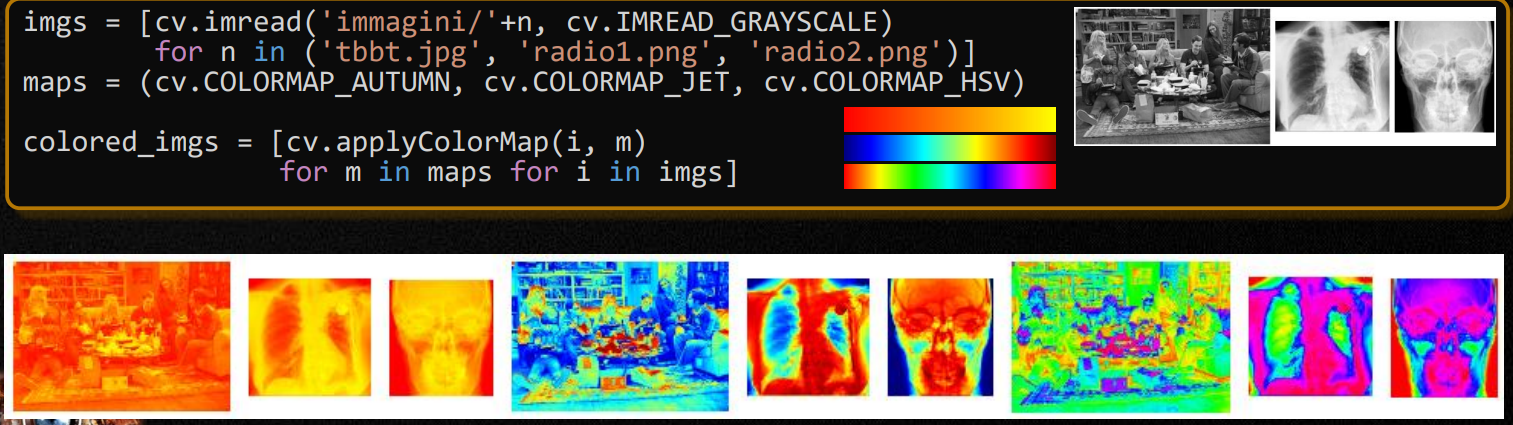
\includegraphics[width=\linewidth]{./immagini/LUT_colored.png}
	\label{img:LUT_colored}
\end{figure}

\section{Operazioni aritmetiche fra immagini}

\subsection{Differenza}

Una operazione comune è la sottrazione dello sfondo ed è molto utile in visione artificiale, permette di catturare ed analizzare porzioni di immagini. Nota: np.nonzero è una funzione che mi ritorna gli indici degli elementi che sono diversi da 0.

\begin{lstlisting}
	#Ho immagine e sfondo, separate. 
	img, back = cv.imread('esempi/mario-game.png'), \ cv.imread('esempi/mario-back.png')
	#Qui fa la differenza bit a bit
	diff = img - back # N.B. diff = cv.subtract(img, back) e' piu' efficiente
	#scelgo tutto cio' che non e' zero, di conseguenza rimane mario
	mask = diff!=0 
	#creo una immagine tutta a zero e dopodiche' applico la maschera
	res = np.zeros_like(img) 
	res[mask] = img[mask]
\end{lstlisting}

\begin{figure}[htp]
	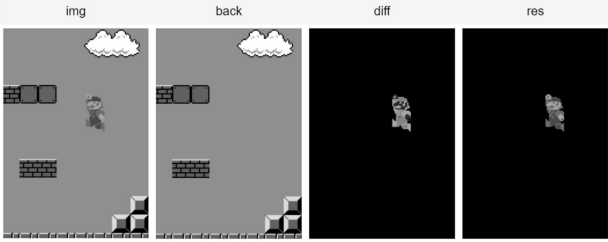
\includegraphics[width=300pt]{./immagini/mario_differenza.png}
	\label{img:mario_differenza}
\end{figure}

\newpage

\subsection{Operazioni bitwise}

\begin{lstlisting}
	sprite = cv.imread('esempi/sprite.png')
	mask = cv.imread('esempi/mask.png')
	back = cv.imread('esempi/hill.jpg')
	res = back.copy()
	x, y = 200, 100
	h, w = sprite.shape[:2]
	#roi = region of interest, pezzettino dello sfondo
	roi = res[y:y+h,x:x+w]
	#questo e' l'AND bit a bit , se faccio l'and con bit a 1 non succede niente, rimane il valore che c'era prima mentre se faccio l'AND con valori a 0 si cancella tutto. Quindi facendo l'and con la maschera nello sfondo, sto andando a lasciare dove c'e' il bianco (riferito alla sprite) lo sfondo, altrimenti c'e' il nero
	roi &= mask	
	#Facendo l'or bit a bit i valori a 0 rimangono tali, gli altri vengono cambiati
	roi |= sprite
\end{lstlisting}

\begin{figure}[htp]
	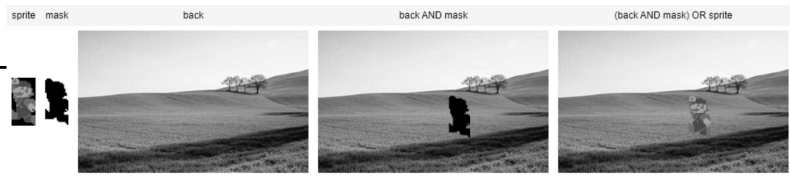
\includegraphics[width=\linewidth]{./immagini/mario_bit.png}
	\label{img:mario_bit}
\end{figure}

\subsection{Alpha blending o aliasing}

Per ottenere un risultato migliore rispetto alle operazioni bitwise ci serve un ulteriore canale, chiamato $\alpha$. Si tratta di un canale che contiene un valore di trasparenza (di solito è un valore floating point fra 0 e 1) e la formula che vado ad applicare corrisponde ad una operazione fra tre immagini, la prima immagine è lo sfondo, la seconda immagine è la sprite e la terza immagine è il canale di trasparenza (è come una maschera, però invece che avere solo il valore 255 e 0, questa può assumere tutti i possibili colori). Come funziona? non si lavora più coi bit, si sfrutta una formula matematica che utilizza i numeri floating point. 

\begin{lstlisting}
	img1 = cv.imread('esempi/hill.jpg')
	img2 = cv.imread('esempi/study.png')
	img2_alpha = cv.imread('esempi/study-alpha.png')
	h, w = img2.shape[:2]
	a = img2_alpha / 255 # Trasforma il canale alpha da [0,255] a [0,1]
	
	x, y = 200, 100
	res = img1.copy()
	res[y:y+h,x:x+w] = img1[y:y+h,x:x+w]*(1.0-a) + img2*a
\end{lstlisting}

\begin{figure}[htp]
	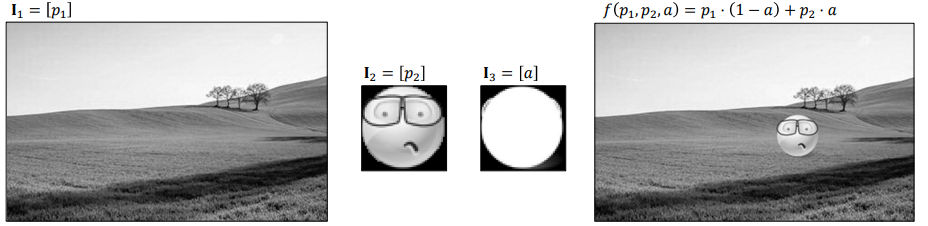
\includegraphics[width=300pt]{./immagini/alpha_blending.png}
	\label{img:alpha_blending}
\end{figure}

\newpage

\section{Binarizzare un'immagine grayscale in opencv}

La binarizzazione consiste nel trasformare una immagine da grayscale ad una con gamma di due colori (generalmente bianco e nero).

\subsection{Soglia globale}
Il metodo più semplice per binarizzare consiste nell'utilizzo di una soglia globale. Una soglia globale è definita dalla seguente funzione:\\
$f(v, t)$ = 
$
\begin{cases}
	0 \quad \quad v < t\\
	255 \quad v \geq t
\end{cases}
$	
\\\\
Il problema dunque è concentrato nella identificazione della soglia... generalmente viene scelta osservando l'istogramma e tracciando una linea di demarcazione fra i due picchi di colore. La soglia si può individuare anche manualmente o attraverso dei metodi, come ad esempio il metodo di Otsu.
\subsubsection{Il metodo di Otsu}

Semplice algoritmo che cerca di trovare quella soglia che va a minimizzare la varianza intra-classe dell'intensità dei pixel delle due classi (una volta effettuata la binarizzazione distinguiamo pixel di background e foreground) determinate dalla soglia stessa. 

\subsection{Soglia locale}
Non sempre una soglia globale può fare al caso nostro, ci sono immagini dove la luce varia in un modo per cui lo sfondo è molto più scuro che in altre. Per risolvere questo problema scelgo più soglie, ad esempio potrei dividere l'immagini in più parti e ad ognuna applicare una diversa soglia. Il metodo più
generale per la soglia locale è quello di avere una soglia diverso per ciascun pixel. 
\subsubsection{Succo del discorso}
La soglia locale è determinata per ogni pixel considerando una piccola regione dell'immagine attorno ad esso. Il metodo più semplice per definirla consiste nel determinare la soglia come media dei pixel nella regione meno un valore costante (openCV ha anche un metodo che sfrutta l'intorno Gaussiano invece che la media).

\newpage

\subsection{Binarizzazione su OpenCV}
OpenCV ci mette a disposizione la funzione treshold, che ci permette di binarizzare una immagine. I parametri che prende sono: l'immagine, il valore della soglia, il valore massimo ed una costante (corrisponde alla soglia globale, posso passare anche OTSU, che ignorerà i parametri). La funzione restituisce una tupla, formata da : valore di ritorno e immagine, il valore di ritorno è la soglia (può tornare utile quando uso OTSU). Per quanto riguarda la binarizzazione con soglia locale OpenCV mette a disposizione la funzione adaptiveThresold, a cui passo (immagine; soglia; costante = tipo di soglia locale; costante = come utilizzo la soglia locale; dimensione della regione di pixel; costante = ciò che sottraggo alla media per ottenere la soglia).


\subsubsection{Chiodi}

\begin{lstlisting}
	# Soglia globale (128)
	img = cv.imread('esempi/bolts.png', cv.IMREAD_GRAYSCALE)
	_, res = cv.threshold(img, 128, 255, cv.THRESH_BINARY)
\end{lstlisting}

\begin{figure}[htp]
	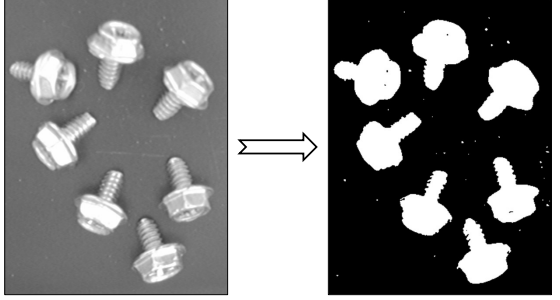
\includegraphics[width=300pt]{./immagini/chiodi_binarizzati.png}
	\label{img:chiodi_binarizzati}
\end{figure}

\subsubsection{Torre}

\begin{lstlisting}
	# Soglia globale determinata dall'algoritmo di Otsu
	img = cv.imread('immagini/torre.jpg', cv.IMREAD_GRAYSCALE)
	t, res = cv.threshold(img, -1, 255, cv.THRESH_OTSU)
\end{lstlisting}

\begin{figure}[htp]
	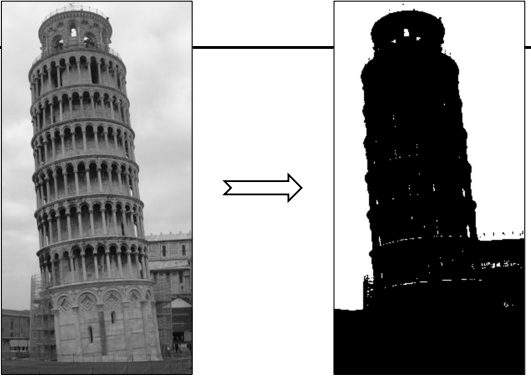
\includegraphics[width=200pt]{./immagini/torre_binarizzata.png}
	\label{img:torre_binarizzata}
\end{figure}

\subsubsection{Sudoku}

\begin{lstlisting}
	# Soglia locale (media su intorno 11x11 meno il valore 10)
	img = cv.imread('immagini/sudoku.jpg', cv.IMREAD_GRAYSCALE)
	res = cv.adaptiveThreshold(img, 255, cv.ADAPTIVE_THRESH_MEAN_C,
	cv.THRESH_BINARY, 11, 10)
\end{lstlisting}

\begin{figure}[htp]
	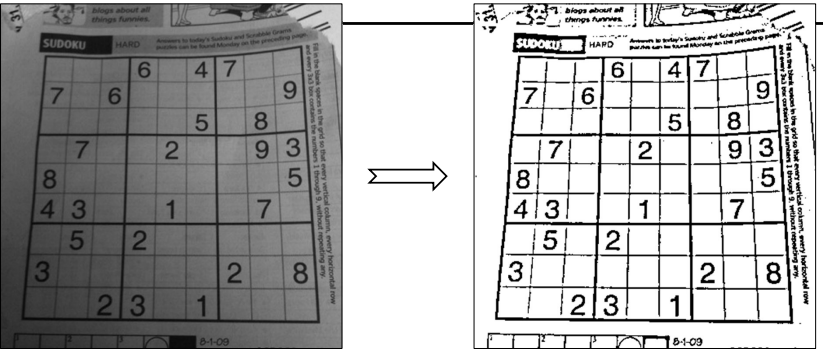
\includegraphics[width=200pt]{./immagini/sudoku_binarizzato.png}
	\label{img:sudoku_binarizzato}
\end{figure}

\subsubsection{Ferrari}

Fino ad ora abbiamo binarizzato delle immagini grayscale, quando abbiamo immagini a colori? posso eventualmente binarizzare i singoli canali, sempre che l'operazione abbia senso. In hls potrebbe essere interessante binarizzare la saturazione, come nell'esempio sottostante.

\begin{lstlisting}
	# Cosa succede binarizzando il canale saturazione di un'immagine HSL?
	img = cv.imread('esempi/ferrari.jpg')
	hls = cv.cvtColor(img, cv.COLOR_BGR2HLS)
	#qui ho sovrascritto la saturazione con la binarizzazione della stessa
	_,hls[...,2] = cv.threshold(hls[...,2], 150, 255, cv.THRESH_BINARY)
	#ho riconvertito da hls a bgr
	res = cv.cvtColor(hls, cv.COLOR_HLS2BGR)
\end{lstlisting}

\begin{figure}[htp]
	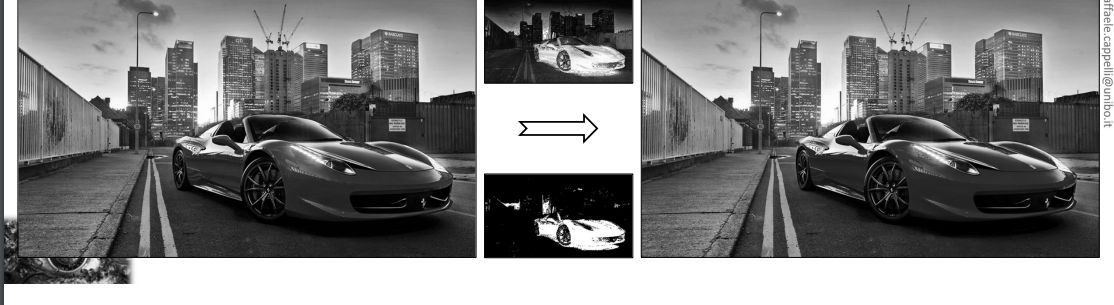
\includegraphics[width=200pt]{./immagini/ferrari_binarizzata.png}
	\label{img:ferrari_binarizzata}
\end{figure}

\section{Contrast stretching}

L'idea del constrast stretching è di migliorare una immagine poco contrastata, ampliando il contrasto, lo si fa espandendo i livelli di grigio. 
\subsubsection{Funzione}
$f(I[y, x]) = 255 \cdot \dfrac{I[y, x] - \alpha}{\beta - \alpha}$\\
 con $\alpha$ = "minimo livello di grigio dell'immagine" e $\beta$ = "massimo livello di grigio dell'immagine. Togliendo il minimo e dividendo per il range cosa verrà fuori, sapendo che $\alpha$ è il minimo di tutti i pixel? Abbiamo che il numeratore della frazione, diviso per il range massimo mi darà sempre un numero compreso fra 0 e 1. Così facendo ho riscalato tutti i miei valori, andando ad allargarli.
 \subsubsection{Problema}
 E' una bella idea, peccato che normalmente non funzioni assolutamente, ma perchè? se c'è anche un solo pixel a zero ed uno solo a 255, la funzione diventa identità, non fa niente dunque. Come risolvo? Considero i bit molto scuri e molto chiari degli outlier, dunque non interessanti. Quindi questo mi permette di ridefinire $\alpha$ e $\beta$, che non necessariamente conterranno il valore minimo o massimo. Posso scegliere ad esempio di scartare il 5 per cento dei pixel più chiari ed il 5 per cento dei pixel più scuri. 

\section{Contrast stretching in Python/OpenCV}

La formula è normalmente implementabile in numpy, l'unico accorgimento è fare in modo che tutti i valori siano float, per fare in modo di calcolare in floating point. Con np.clip, effettuo un troncamento e forzo il risultato chiudendo il range da 0 a 255. Per la trovata del percentile sfrutto la funzione np.percentile per  definire $\alpha$ e $\beta$.

\begin{lstlisting}
	def contrast_stretching(img, a, b):
		
		# Converte in floating point
		n = 255*(img.astype(float)-a)/(b-a)
		
		# Forza il range [0,255] e converte in byte
		return np.clip(n, 0, 255).astype(np.uint8)
	
	img = cv.imread('immagini/rice.png', cv.IMREAD_GRAYSCALE)
	
	# Contrast stretching con alfa=min(I) e beta=max(I)
	res = contrast_stretching(img, img.min(), img.max())
	img = cv.imread('esempi/kernel.png', cv.IMREAD_GRAYSCALE)
	
	# Contrast stretching con alfa=P_5(I) e beta=P_95(I)
	res = contrast_stretching(img, np.percentile(img, 5), np.percentile(img, 95))
\end{lstlisting}

\section{Equalizzazione dell'istogramma}

Altro modo per migliorare il contrasto, il vantaggio rispetto al constrast stretching è che non ha parametri, quindi gli passo l'immagine e fa quello che deve fare (non è detto che sia meglio rispetto allo stretching, dipende dal constesto). Si sfrutta spesso per migliorare il contrasto o rendere confrontabili immagini catturate in condizioni diverse di illuminazione.

\subsection{Funzionamento}

L'equalizzatore vuole distribuire tutti i livelli di grigio dell'istogramma in maniera uniforme. Zone dell'istogramma che sono scarsamente popolate, ovvero con pochi pixel, vengono compresse mentre le zone con molti pixel vengono allargate. Vogliamo dare più sfumature di grigio, aumentando il contrasto dove c'è più concentrazione di pixel e diminuendolo nelle zone meno popolate.

\subsection{Formula}

$f(v) = \sum_{i = 0}^{v}H[i]$\\\\Con H istogramma dell'immagine normalizzato:
$H[i] = \dfrac{255 \cdot h[i]}{\sum h[i]} \rightarrow \sum_{i = 0}^{255}H[i] = 255$


\section{Equalizzazione a colori}

Posso effettuare l'equalizzazione anche sull'immagine a colori. Attenzione perchè non ha senso equalizzare separatamente i canali RGB, certi colori cambiano, non è più la stessa immagine.
\paragraph{Ha senso} convertire in HSL e equalizzare solo sul canale della luminosità.

\section{Equalizzazione in OpenCV}



\begin{lstlisting}
	#Equalizzazione di un'immagine grayscale
	img = cv.imread('esempi/kernel.png', cv.IMREAD_GRAYSCALE)
	res = cv.equalizeHist(img) #lavora su immagini grayscale
	
	# Equalizzazione di un'immagine a colori
	# Esempio di come NON fare: equalizzazione di ciascun canale RGB
	bgr = cv.imread('immagini/tbbt.jpg')
	b, g, r = cv.split(bgr)
	b_eq, g_eq, r_eq = [cv.equalizeHist(x) for x in (b, g, r)]
	res_wrong = cv.merge((b_eq, g_eq, r_eq))
	
	# Esempio di come procedere convertendo in HSL ed equalizzando L
	hls = cv.cvtColor(bgr, cv.COLOR_BGR2HLS)
	h, l, s = cv.split(hls)
	l_eq = cv.equalizeHist(l)
	hls_eq = cv.merge((h, l_eq, s))
	res_ok = cv.cvtColor(hls_eq, cv.COLOR_HLS2BGR)
\end{lstlisting}
	
	\chapter{Calibrazione}

\begin{lstlisting}
	//Hello.java
	import javax.swing.JApplet;
	import java.awt.Graphics;
	
	public class Hello extends JApplet {
		public void paintComponent(Graphics g) {
			g.drawString("Hello, world!", 65, 95);
		}    
	}
\end{lstlisting}
	
	\chapter{Filtri}

\begin{lstlisting}
	//Hello.java
	import javax.swing.JApplet;
	import java.awt.Graphics;
	
	public class Hello extends JApplet {
		public void paintComponent(Graphics g) {
			g.drawString("Hello, world!", 65, 95);
		}    
	}
\end{lstlisting}
	
	\chapter{Analisi}

\begin{lstlisting}
	//Hello.java
	import javax.swing.JApplet;
	import java.awt.Graphics;
	
	public class Hello extends JApplet {
		public void paintComponent(Graphics g) {
			g.drawString("Hello, world!", 65, 95);
		}    
	}
\end{lstlisting}
	
	\chapter{Movimento}

\begin{lstlisting}
	//Hello.java
	import javax.swing.JApplet;
	import java.awt.Graphics;
	
	public class Hello extends JApplet {
		public void paintComponent(Graphics g) {
			g.drawString("Hello, world!", 65, 95);
		}    
	}
\end{lstlisting}
	
	% ---------------------------------- RICONOSCIMENTO -------------------------------------
\chapter{Riconoscimento}

\begin{lstlisting}
	//Hello.java
	import javax.swing.JApplet;
	import java.awt.Graphics;
	
	public class Hello extends JApplet {
		public void paintComponent(Graphics g) {
			g.drawString("Hello, world!", 65, 95);
		}    
	}
\end{lstlisting}
	

\end{document}